\documentclass[a4j,10pt,dvipdfmx]{jarticle}
\usepackage{url}
\usepackage[version=3]{mhchem}
\usepackage{siunitx}
\usepackage[dvipdfmx]{graphicx}
\usepackage{pdfpages}
\usepackage{here}
\author{学籍番号2120029, 氏名 政野玄空}
\date{2023年5月20日}
\begin{document}
\title{事前課題}
\maketitle
\section{実験課題(1)の測定結果である$I_C$ - $V_{CE}$ 特性、$I_C$ - $I_B$ 特性、$I_B$ - $V_{BE}$ 特性の測定データ
を表にまとめ、グラフ化する。}
\begin{table}[H]
\label{1}
\begin{center}
\caption{$V_{CE}$が4Vのときの$I_C$ - $I_B$,$I_B$ - $V_{BE}$特性}
\begin{tabular}{cccc} \\
\hline
$I_B$[µA] & $I_C$[mA] & $V_{BE}$[V] & $V_{CE}$[V] \\
17 & 0 & 0 & 0 \\
0.000  & 0.000  & 0.001  & 4.001  \\
0.020  & 0.000  & 0.298  & 4.001  \\
0.250  & 0.030  & 0.570  & 3.998  \\
2.603  & 0.382  & 0.640  & 3.962  \\
5.405  & 0.806  & 0.660  & 3.918  \\
8.293  & 1.245  & 0.670  & 3.873  \\
11.210  & 1.691  & 0.678  & 4.020  \\
14.157  & 2.139  & 0.683  & 3.981  \\
17.106  & 2.589  & 0.688  & 3.935  \\
20.059  & 3.039  & 0.692  & 3.889  \\
23.020  & 3.490  & 0.696  & 3.943  \\
25.988  & 3.944  & 0.699  & 3.896  \\
28.959  & 4.398  & 0.701  & 3.850  \\
31.932  & 4.854  & 0.704  & 4.003  \\
34.909  & 5.328  & 0.706  & 4.486  \\
37.887  & 5.774  & 0.708  & 3.986  \\
40.869 & 6.231 & 0.709 & 3.984 \\
 \hline
\end{tabular}
\end{center}
\end{table}
\begin{table}[H]
\label{2}
\begin{center}
\caption{$I_B$が30[µA]のときの$I_C$ - $V_{CE}$特性}
\begin{tabular}{ccc} \\
\hline
IB[µA] & IC[mA] & VCE[V] \\ \hline
30.020  & 0.018  & 0.005  \\
30.059  & 1.088  & 0.089  \\
29.834  & 2.616  & 0.133  \\
29.726  & 3.970  & 0.194  \\
29.714  & 4.390  & 0.351  \\
29.708  & 4.410  & 0.549  \\
29.712  & 4.433  & 1.147  \\
29.714  & 4.446  & 1.545  \\
29.722  & 4.474  & 2.542  \\
29.727  & 4.503  & 3.539  \\
29.740  & 4.547  & 5.534  \\
29.755  & 4.604  & 7.528  \\
29.780  & 4.653  & 9.522  \\
29.808  & 4.704  & 11.518  \\
29.822  & 4.732  & 12.015  \\ \hline
\end{tabular}
\end{center}
\end{table}
\begin{table}[H]
\label{3}
\begin{center}
\caption{$I_B$が20[µA]のときの$I_C$ - $V_{CE}$特性}
\begin{tabular}{ccc} \\
\hline
IB[µA] & IC[mA] & VCE[V] \\ \hline
20.094  & 0.0015 & 0.003 \\
19.242  & 0.962  & 0.102  \\
20.000  & 2.351  & 0.160  \\
19.956  & 2.951  & 0.299  \\
19.952  & 2.964  & 0.497  \\
19.953  & 2.971  & 0.696  \\
19.956  & 2.975  & 0.896  \\
19.956  & 2.983  & 1.295  \\
19.958  & 2.988  & 1.494  \\
19.960  & 2.992  & 1.694  \\
19.962  & 3.006  & 2.693  \\
19.970  & 3.034  & 4.689  \\
19.991  & 3.068  & 6.686  \\
20.006  & 3.105  & 9.681  \\
20.029  & 3.137  & 11.678  \\
20.034  & 3.145  & 12.070  \\ \hline
\end{tabular}
\end{center}
\end{table}
\begin{table}[H]
\label{4}
\begin{center}
\caption{$I_B$が10[µA]のときの$I_C$ - $V_{CE}$特性}
\begin{tabular}{ccc} \\
\hline
IB[µA] & IC[mA] & VCE[V] \\ \hline
10.387 & 0.0085 & 0.002 \\
10.361 & 0.2338 & 0.077 \\
10.0725 & 0.767 & 0.122 \\
9.944 & 1.274 & 0.171 \\
9.912 & 1.456 & 0.252 \\
9.912 & 1.468 & 0.351 \\
9.912 & 1.47 & 0.45 \\
9.912 & 1.471 & 0.55 \\
9.913 & 1.472 & 0.65 \\
9.912 & 1.474 & 0.75 \\
10.234 & 1.522 & 0.845 \\
10.235 & 1.529 & 1.844 \\
10.236 & 1.535 & 2.843 \\
10.239 & 1.541 & 3.843 \\
10.242 & 1.547 & 4.842 \\
10.245 & 1.552 & 5.841 \\
10.25 & 1.559 & 6.84 \\
10.255 & 1.564 & 7.84 \\
10.26 & 1.57 & 8.83 \\
10.262 & 1.574 & 9.838 \\
10.264 & 1.579 & 10.838 \\
10.267 & 1.584 & 11.838 \\
10.252 & 1.584 & 12.056 \\ \hline
\end{tabular}
\end{center}
\end{table}
\begin{figure}[H]
  \begin{center}
  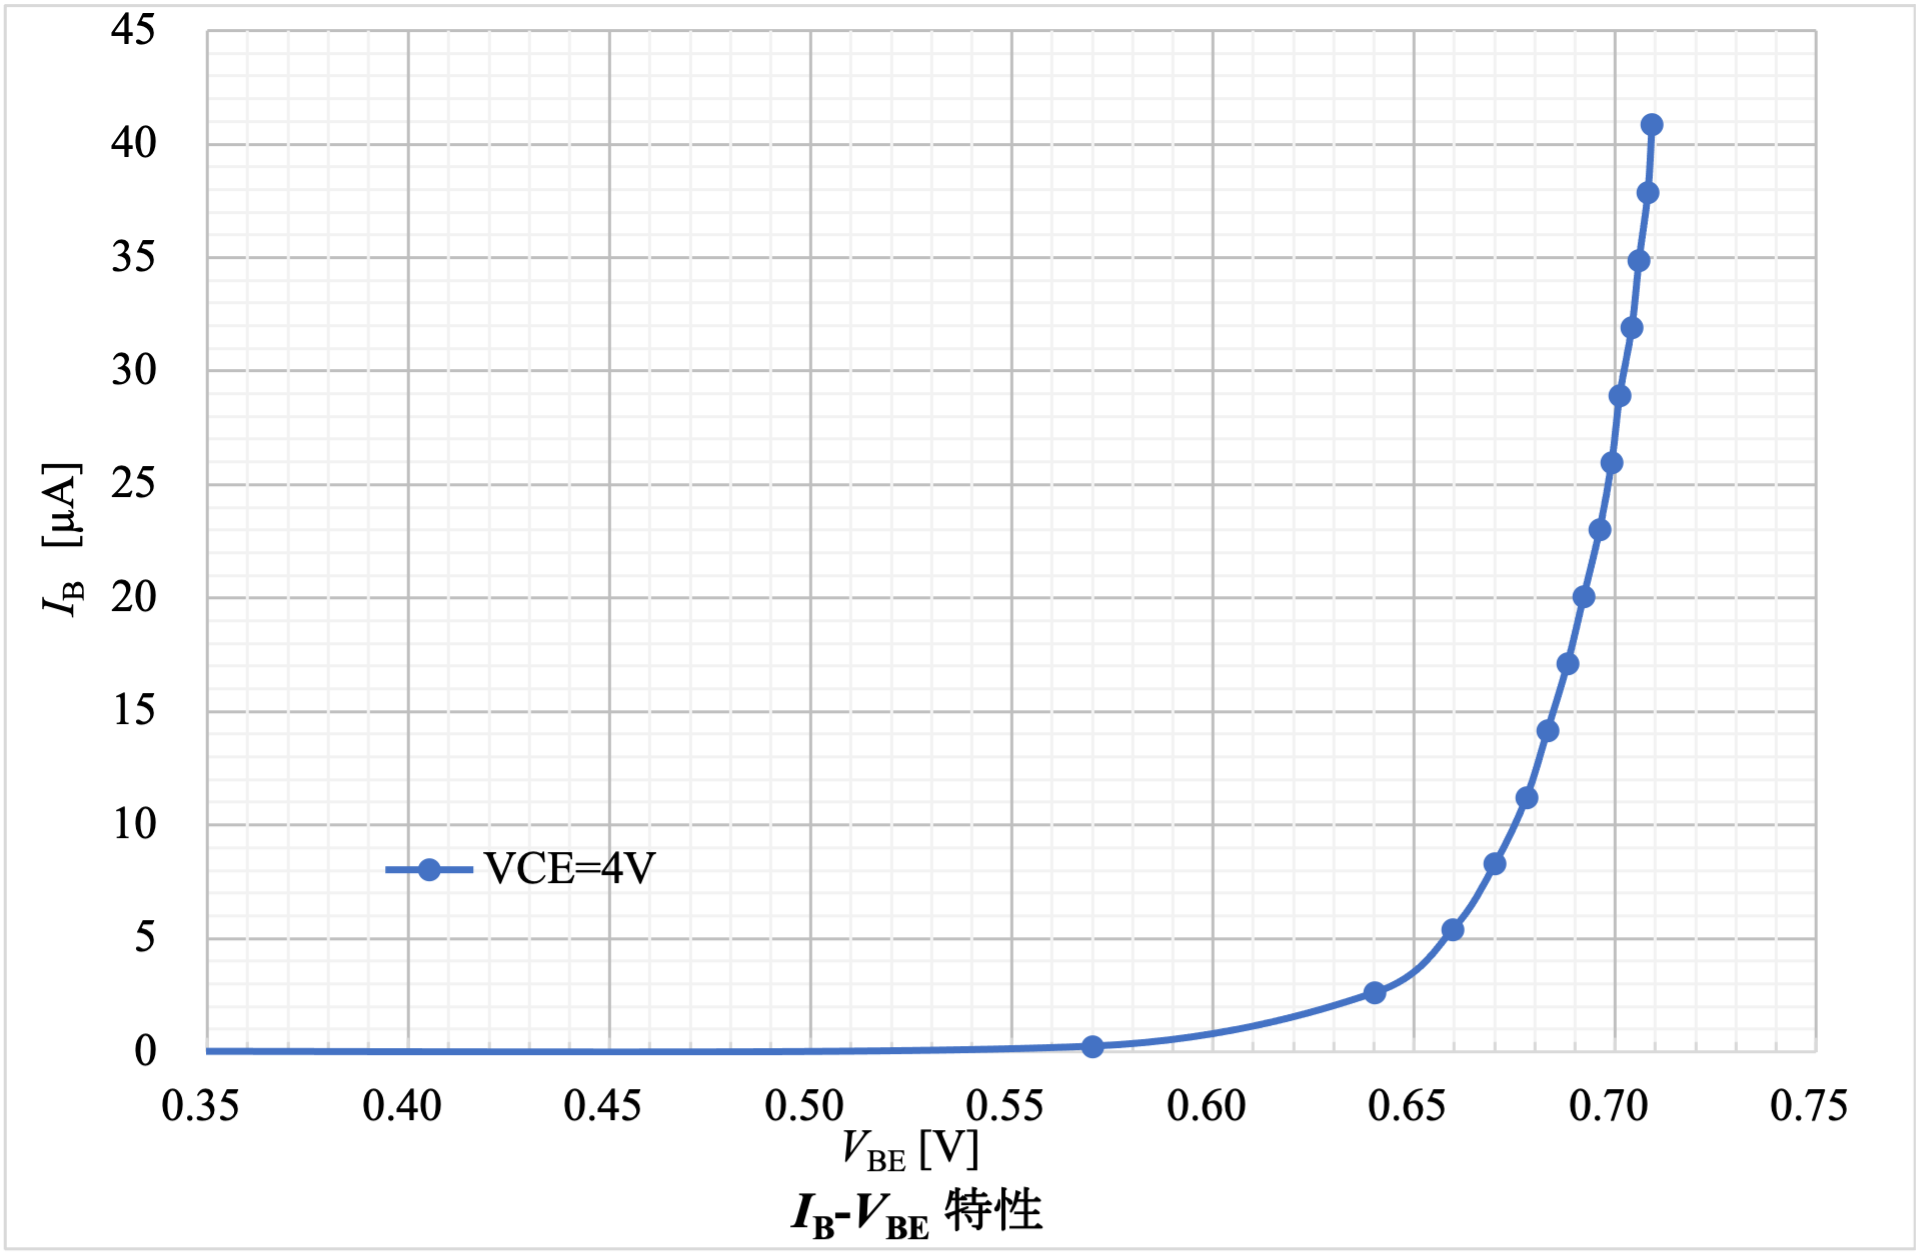
\includegraphics[height=7cm,width=10cm]{4vibvbe.png}
  \caption{$V_{CE}$が4Vのときの$I_B$ - $V_{BE}$特性}
\end{center}
\end{figure}
\begin{figure}[H]
  \begin{center}
  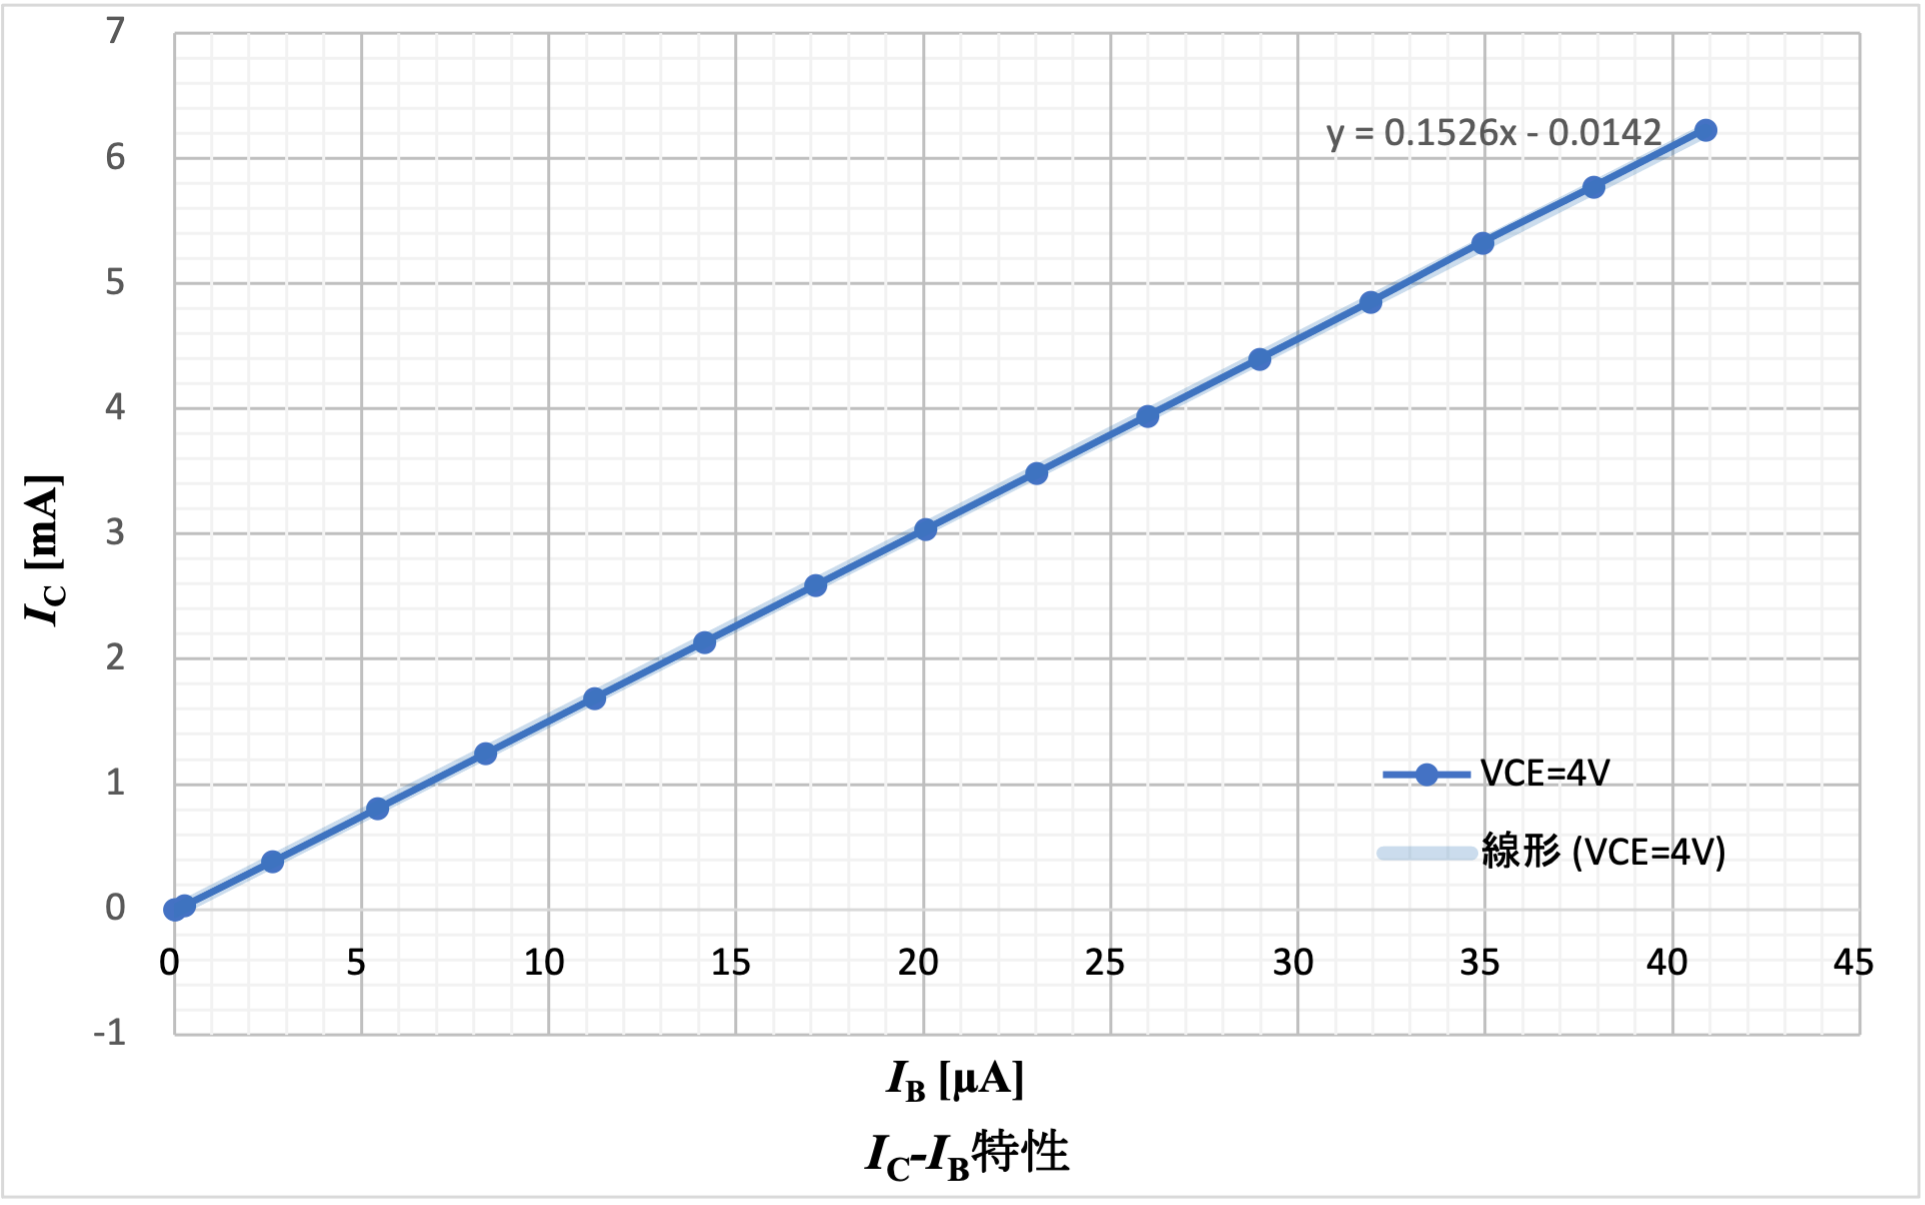
\includegraphics[height=7cm,width=10cm]{v4icib.png}
  \caption{$V_{CE}$が4Vのときの$I_C$ - $I_B$特性}
\end{center}
\end{figure}
\begin{figure}[H]
  \begin{center}
  \label{1030}
  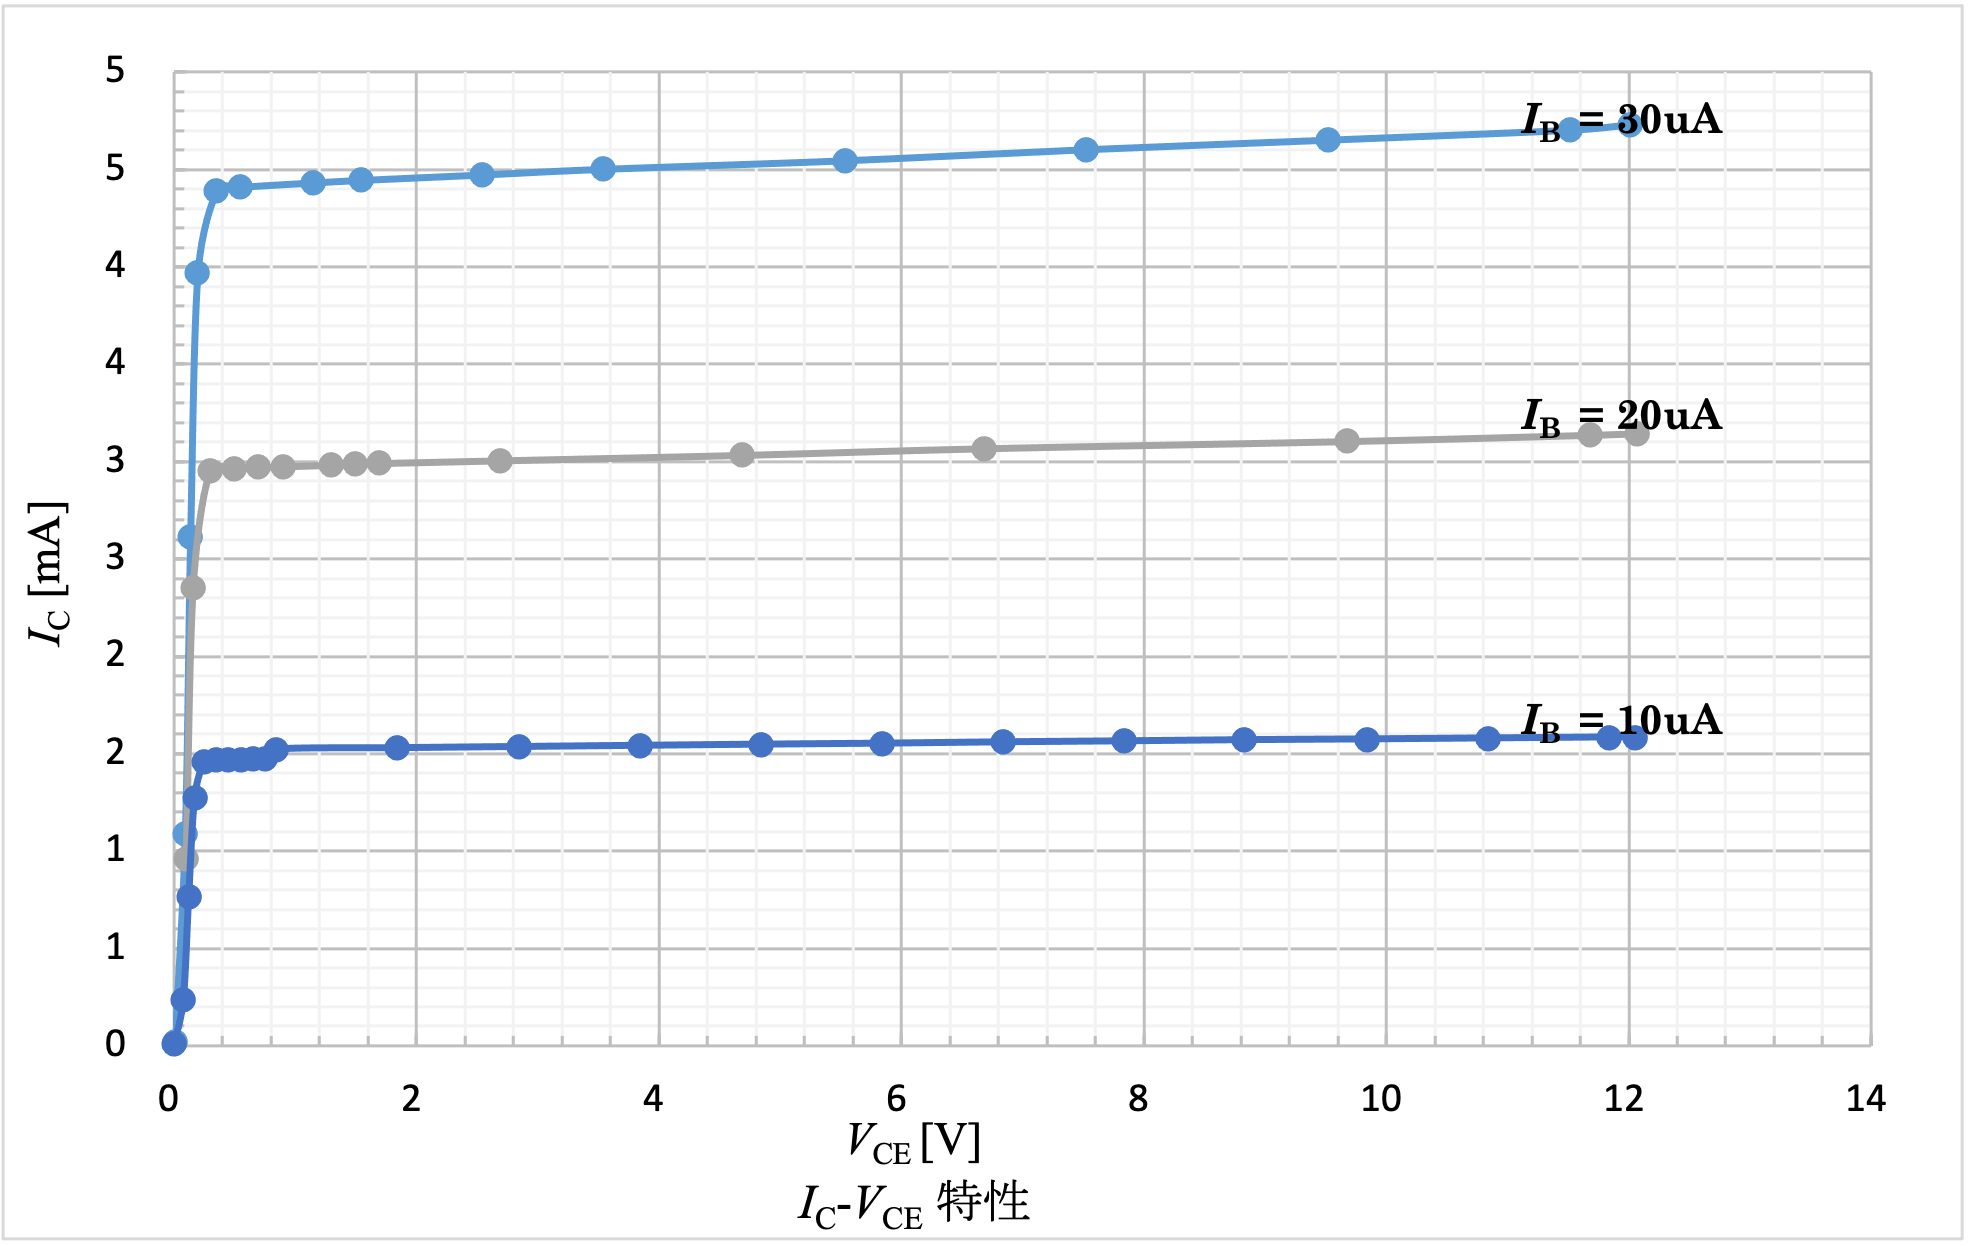
\includegraphics[height=7cm,width=10cm]{icvce1030.png}
  \caption{$I_B$が10[µA],20[µA],30[µA]のときの$I_C$ - $V_{CE}$特性}
\end{center}
\end{figure}
\section{2.2 (3)手順1を参照し、測定した$I_C$―$I_B$ 特性から$I_B$=20 μA 前後のデータを用いて
$h_{FE}$ と$h_{fe}$ を求める。また2.2 (3)手順3を参照し、同$I_B$ 付近のデータを用いて$I_B$ - $V_{BE}$
特性から$h_{ie}$ を求める。}
(\ref{1})より,20μAあたりは$I_C$=3.039,$I_B$=20.059となるので

\begin{eqnarray}
  \label{hFE}
  h_{FE}=\frac{3.039}{20.059\times10^{-3}}=151.5[mA]
\end{eqnarray}
同様に(\ref{1})より,$I_{C2}$=4.854,$I_{B2}$=31.932,$I_{C1}$=1.691,$I_{B1}$=11.210となり
\begin{eqnarray}
  \label{hfe}
  h_{fe}=\frac{4.854-1.691}{31.932-11.210\times10^{-3}}=152.6[mA]
\end{eqnarray}
となる.
つづいて$h_{ie}$ を求める.$A_V$は\cite{a}の表2.1より150,$R_C$は\cite{a}の(2.5)と表2.1より2.2kΩ,$h_{fe}$は(\ref{hfe})で求めたので,\cite{a}の(2.6)より

\begin{eqnarray}
  \label{hie}
  h_{ie}=\frac{150\times{2200}}{150}=2238.13[mA]
\end{eqnarray}
\cite{a}の(2.7)より,$I_{B2}$=31.932,$I_{B1}$=11.210,$V_{BE2}$=0.704,$V_{BE1}$=0.678となり
\begin{eqnarray}
  \label{hie2}
  h_{ie}=\frac{0.704-0.678}{31.932-11.210\times10^{-3}}=1254.71[mA]
\end{eqnarray}

\section{結果より 2.2 (3)を参照し、電流帰還型バイアス回路について各素子の定数を設計す
る。}
電流帰還型バイアス回路について各素子の定数を設計する.

\begin{thebibliography}{9}
  \bibitem{a} 電気通信大学『アナログ回路実験』2023年,p10$\sim$15
\end{thebibliography}
\end{document}
